\chapter*{Dodatak: Prikaz aktivnosti grupe}
		\addcontentsline{toc}{chapter}{Dodatak: Prikaz aktivnosti grupe}
		
		\section*{Dnevnik sastajanja}
		
		
		
		\begin{packed_enum}
			\item  sastanak
			
			\item[] \begin{packed_item}
				\item Datum: 12. listopada 2021. 
				\item Prisustvovali: M.Damjanić, F.Tomljenović, I.Jeržabek, A.Griparić, R.Mihalić
				\item Teme sastanka:
				\begin{packed_item}
					\item  Moguće alternativne ideje za projekt
					\item  Početne ideje za tehnologije
				\end{packed_item}
			\end{packed_item}
			
			\item  sastanak
			\item[] \begin{packed_item}
				\item Datum: 14. listopada 2021. 
				\item Prisustvovali: M.Damjanić, F.Tomljenović, I.Jeržabek, A.Griparić, R.Mihalić, L.Maros, F.Jelavić
				\item Teme sastanka:
				\begin{packed_item}
					\item  Dogovorene korištene tehnologije
				\end{packed_item}
			\end{packed_item}
		
			\item  sastanak
			\item[] \begin{packed_item}
				\item Datum: 28. listopada 2021. 
				\item Prisustvovali: M.Damjanić, F.Tomljenović, I.Jeržabek, A.Griparić, R.Mihalić, L.Maros, F.Jelavić
				\item Teme sastanka:
				\begin{packed_item}
					\item  Predložen koncept cijelog projekta
					\item  Podjela posla po članovima za 1.ciklus
				\end{packed_item}
			\end{packed_item}
		
			\item  sastanak
			\item[] \begin{packed_item}
				\item Datum: 12. studeni 2021. 
				\item Prisustvovali: M.Damjanić, F.Tomljenović, I.Jeržabek, A.Griparić, R.Mihalić, L.Maros, F.Jelavić
				\item Teme sastanka:
				\begin{packed_item}
					\item  Jeržabek je održao predavanje o Reactu
					\item  Dane upute o spajanju na bazu i pisanju dokumentacije
				\end{packed_item}
			\end{packed_item}
			
			\eject
			\item  sastanak
			\item[] \begin{packed_item}
				\item Datum: 17. studeni 2021. 
				\item Prisustvovali: M.Damjanić, I.Jeržabek, A.Griparić, R.Mihalić
				\item Teme sastanka:
				\begin{packed_item}
					\item   Sastanak s asistentom i demosom - evaluacija dosadašnjeg rada
				\end{packed_item}
			\end{packed_item}
		
			\item  sastanak
			\item[] \begin{packed_item}
				\item Datum: 8. prosinca 2021. 
				\item Prisustvovali: M.Damjanić, F.Tomljenović, I.Jeržabek, A.Griparić, R.Mihalić, L.Maros, F.Jelavić
				\item Teme sastanka:
				\begin{packed_item}
					\item  Prolaženje kroz svih dijelova projekta sa svim članovima
				\end{packed_item}
			\end{packed_item}
		
			\item  sastanak
			\item[] \begin{packed_item}
				\item Datum: 16. prosinca 2021. 
				\item Prisustvovali: M.Damjanić, F.Tomljenović, I.Jeržabek, A.Griparić, R.Mihalić, L.Maros
				\item Teme sastanka:
				\begin{packed_item}
					\item  Dogovorene raspodjela poslova za 2.ciklus
				\end{packed_item}
			\end{packed_item}
		
			\item  sastanak
			\item[] \begin{packed_item}
				\item Datum: 21. prosinac 2021. 
				\item Prisustvovali: F.Tomljenović, I.Jeržabek, A.Griparić, R.Mihalić, L.Maros
				\item Teme sastanka:
				\begin{packed_item}
					\item   sastanak s asistentom i demosom - demonstracija alfa inačice
				\end{packed_item}
			\end{packed_item}
		
			\item  sastanak
			\item[] \begin{packed_item}
				\item Datum: 13. siječnja 2022. 
				\item Prisustvovali: M.Damjanić, I.Jeržabek, R.Mihalić
				\item Teme sastanka:
				\begin{packed_item}
					\item  sastanak s asistentom za zadnje implementacije i izvođenje buduće prezentacije
				\end{packed_item}
			\end{packed_item}			
			%
			
		\end{packed_enum}
		
		\eject
		\section*{Tablica aktivnosti}
		
			

			\begin{longtblr}[
					label=none,
				]{
					vlines,hlines,
					width = \textwidth,
					colspec={X[7, l]X[1, c]X[1, c]X[1, c]X[1, c]X[1, c]X[1, c]X[1, c]}, 
					vline{1} = {1}{text=\clap{}},
					hline{1} = {1}{text=\clap{}},
					rowhead = 1,
				} 
				\multicolumn{1}{c|}{} & \multicolumn{1}{c|}{\rotatebox{90}{\textbf{Marko Damjanić}}} & \multicolumn{1}{c|}{\rotatebox{90}{\textbf{Ivan Jeržabek}}} &	\multicolumn{1}{c|}{\rotatebox{90}{\textbf{Roko Mihalić}}} & \multicolumn{1}{c|}{\rotatebox{90}{\textbf{Fran Tomljenović}}} &	\multicolumn{1}{c|}{\rotatebox{90}{\textbf{Fran Jelavić}}} & \multicolumn{1}{c|}{\rotatebox{90}{\textbf{Antonio Griparić}}} &	\multicolumn{1}{c|}{\rotatebox{90}{\textbf{Luka Maros}}} \\  
				Upravljanje projektom 		& 25  &  &  &  &  &  & \\ 
				Opis projektnog zadatka 	& 6  &  &  &  &  &  & \\ 
				
				Funkcionalni zahtjevi       &  &  &  &  & 5 &  &  \\ 
				Opis pojedinih obrazaca 	&  &  &  &  &  & 10 & 10 \\ 
				Dijagram obrazaca 			&  &  &  &  &  & 4 &  \\ 
				Sekvencijski dijagrami 		&  &  &  &  &  &  & 4 \\ 
				Opis ostalih zahtjeva 		& 1 &  &  &  &  &  &  \\ 

				Arhitektura i dizajn sustava	 &  &  &  &  & 5 &  &  \\ 
				Baza podataka				& 15 &  & 5 & 5 &  &  &   \\ 
				Dijagram razreda 			&  &  & 3 &  &  &  &   \\ 
				Dijagram stanja				& 3 &  &  &  &  &  &  \\ 
				Dijagram aktivnosti 		& 2 &  &  &  &  &  &  \\ 
				Dijagram komponenti			&  &  &  &  &  &  &  \\ 
				Korištene tehnologije i alati 		& 1 & 1 & 1 &  &  &  &  \\ 
				Ispitivanje programskog rješenja & 1 &  & 8 &  &  &  &  \\ 
				Dijagram razmještaja			& 1 &  &  &  &  &  &  \\ 
				Upute za puštanje u pogon 		& 2 & 2 & 2 &  &  &  &  \\  
				Dnevnik sastajanja 			& 2 &  &  &  &  &  &  \\ 
				Zaključak i budući rad 		& 1 &  &  &  &  &  &  \\  
				Popis literature 			& 1 &  &  &  &  &  &  \\  
				Izrada početne stranice		&  &  &  &  & 15  &  &  \\ 
				Izrada stranice s zadacima	&  & 2 &  &  &  & 15 &  \\ 
				Izrada stranice odabranog zadatka &  & 2 &  &  &  & 15 &  \\  
			 	Izrada stranice natjecanja		&  & 50 &  &  &  &  &  \\ 
			 	Izrada stranice korisničkih profila	&  & 3 &  &  &  &  & 35 \\ 
			 	Izrada stranice članova &  & 2 &  &  & 15 &  &  \\ 
			 	Izrada baze podataka & 20 &  &  &  &  &  &  \\ 
				Back end		&  &  & 120 & 100 &  &  &  \\  
				Puštanje u pogon &  & 35 &  & 5 &  &  &\\ 
				 							
			\end{longtblr}
					
					
		\eject
		\section*{Dijagrami pregleda promjena}
		
		\begin{figure}[H]
			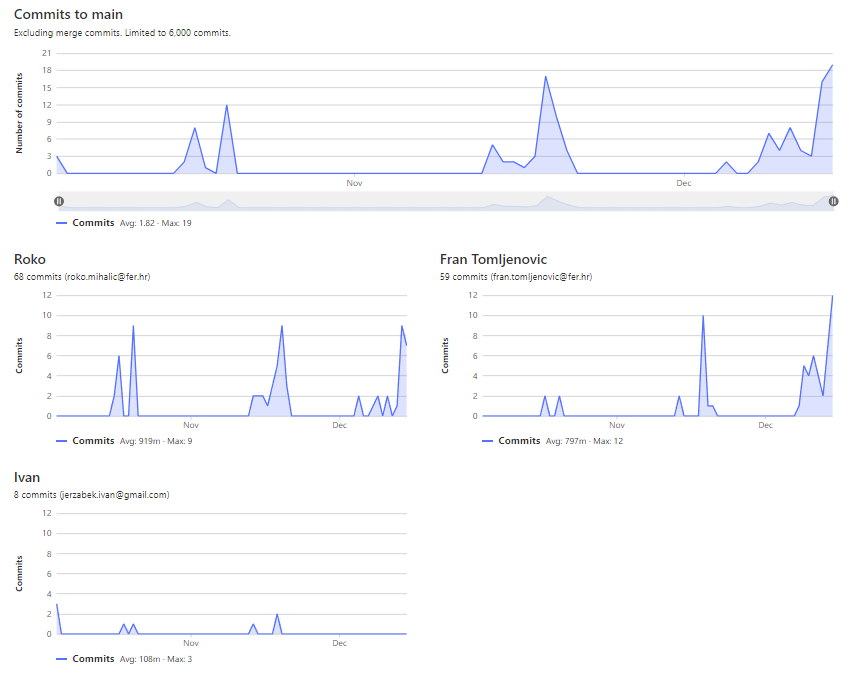
\includegraphics[width=\textwidth]{slike/PrikazAktivnostiNaRepozitorijuPrviDio.png} %veličina u odnosu na širinu linije
			\caption{Prikaz Aktivnosti Na Repozitoriju Prvi Dio}
			\label{fig:PrikazAktivnostiNaRepozitorijuPrviDio} %label mora biti drugaciji za svaku sliku
		\end{figure}
		
		\begin{figure}[H]
			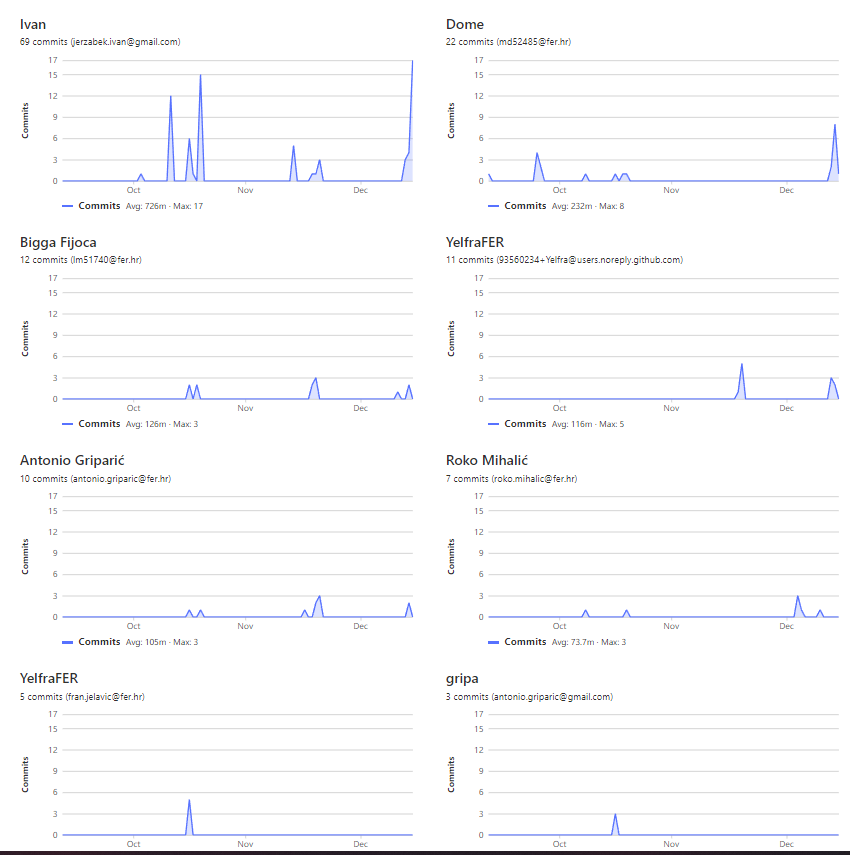
\includegraphics[width=\textwidth]{slike/PrikazAktivnostiNaRepozitorijuDrugiDio.png} %veličina u odnosu na širinu linije
			\caption{Prikaz Aktivnosti Na Repozitoriju Drugi Dio}
			\label{fig:PrikazAktivnostiNaRepozitorijuDrugiDio} %label mora biti drugaciji za svaku sliku
		\end{figure}
	
		
	